%% Adapted from GaTech CS 7545 Machine Learning Theory given by Prof. Jacob Abernathy Fall 2018. Original latex file: https://github.com/mltheory/CS7545/blob/master/scribe/CS7545scribe_template.tex 



%%%%%PLEASE CONSIDER CORRECTIONS AT PLACES INDICATED%%%%%%%%
\documentclass{article}
%%%%%Packages Used, add more if necessary%%%%
\usepackage{amsmath,amsfonts,amssymb,graphicx,fullpage, float}
\setlength{\topmargin}{-0.6 in}
\setlength{\textheight}{8.5 in}
\setlength{\headsep}{0.75 in}
\usepackage{mdframed}
\usepackage{multicol}
\usepackage{microtype}
\usepackage{animate}
\usepackage{amsmath}
\usepackage{float}
\usepackage{url, hyperref}
\usepackage{breakurl}



%%%%% NO NEED TO EDIT THIS PREAMBLE %%%%%%%%
%%% PREAMBLE %%%
\newcounter{lecnum}
\renewcommand{\thepage}{\thelecnum-\arabic{page}}
\renewcommand{\thesection}{\thelecnum.\arabic{section}}
\renewcommand{\theequation}{\thelecnum.\arabic{equation}}
\renewcommand{\thefigure}{\thelecnum.\arabic{figure}}
\renewcommand{\thetable}{\thelecnum.\arabic{table}}
\newcommand{\lecture}[4]{
   \pagestyle{myheadings}
   \thispagestyle{plain}
   \newpage
   \setcounter{lecnum}{#1}
   \setcounter{page}{1}
   \noindent
   \begin{center}
   \framebox{
      \vbox{\vspace{2mm}
      
      \hbox to 6.28in { 
      {\bf ECE 4252/6252 (FunML) Fundamentals of Machine Learning \hfill 2021--2028} }
      
      \vspace{2mm}
      \hbox to 6.28in { 
      {Courses developed by Professor Ghassan AlRegib 
      (\href{https://alregib.ece.gatech.edu/}{alregib.ece.gatech.edu}) 
      \hfill For inquiries: \href{mailto:alregib@gatech.edu}{alregib@gatech.edu}} }
      
      \vspace{3mm}
      \hbox to 6.28in { {\Large \hfill Lecture #1: #2 \hfill} }
      
      \vspace{2mm}
      \hbox to 6.28in { {\it Co-Instructors: #3 \hfill #4} }
      
      \vspace{2mm}}
   }
   \end{center}

   % -------- PEOPLE OUTSIDE BOX --------
   \vspace{2mm}
   \noindent{\bf Contributors:} Dr. Ahmad Mustafa, Dr. Motaz Alfarraj, Dr. Ashraf Alattar, Dr. Chen Zhou

   \vspace{1mm}
   \noindent{\bf Teaching Assistants} with remarkable contributions include: Kuo-Wei Lai, Wuyang Du, Shiva Mahato, Michael Zhou, Ninghan Zhong

   \markboth{Lecture #1: #2}{Lecture #1: #2}

   \vspace{2mm}
\noindent {\bf Disclaimer}: 
{All content of these notes are part of this course at Georgia Tech. Any re-use or distribution is not permitted without pre-approved permission. All these notes belong to, created by, and copyrighted for Ghassan AlRegib and Mohit Prabhushankar, Georgia Tech, 2021--2028.}

\vspace{2mm}
\noindent {\bf License}: 
{These lecture notes are licensed under the 
\href{https://creativecommons.org/licenses/by-nc-sa/4.0/}{Creative Commons Attribution-NonCommercial-ShareAlike 4.0 International License}.}

   \vspace{2mm}
   \noindent {\bf Errata}: 
   {\it Please submit any errata you find using the following form: 
   \href{https://forms.office.com/r/fbg9dMWPgY}{Errata Form for FunML Textbook} 
   or visit: \url{https://forms.office.com/r/fbg9dMWPgY}}

   \vspace*{4mm}
}
\renewcommand{\cite}[1]{[#1]}
\def\beginrefs{\begin{list}
        {[\arabic{equation}]}{\usecounter{equation}
         \setlength{\leftmargin}{2.0truecm}\setlength{\labelsep}{0.4truecm}%
         \setlength{\labelwidth}{1.6truecm}}}
\def\endrefs{\end{list}}
\def\bibentry#1{\item[\hbox{[#1]}]}

\newcommand{\challenge}[2]{\noindent \textbf{(Challenge Problem)} \emph{#1}: #2 }

\newcommand{\exercise}[1]{\noindent \textbf{(Exercise)} #1 }

\newcommand{\fig}[3]{
			\vspace{#2}
			\begin{center}
			Figure \thelecnum.#1:~#3
			\end{center}
	}
%%% END_OF_PREAMBLE %%%


	
%%%%You may add more \newtheorem if necessary%%%%%%
\newtheorem{theorem}{Theorem}[lecnum]
\newtheorem{lemma}[theorem]{Lemma}
\newtheorem{proposition}[theorem]{Proposition}
\newtheorem{claim}[theorem]{Claim}
\newtheorem{corollary}[theorem]{Corollary}
\newtheorem{definition}[theorem]{Definition}
\newenvironment{proof}{{\bf Proof:}}{\hfill\rule{2mm}{2mm}}


\newcommand{\dom}{\mathrm{dom}}
\begin{document}

%%%%%CHANGE HERE%%%%%%%
%%%%%\section{title of the section} similarly with the rest \section{} or \subsection{} or \subsubsection{} etc


%%%%%CHANGE HERE%%%%%%%%%
%%%%%\lecture{the ordinal number of the lecture}{lecture title}{Jacob Abernethy}{scriber's name}%%%%%%%%
\lecture{18}{Autoencoder Extensions}{Ghassan AlRegib and Mohit Prabhushankar}{}%%

%%%%%CHANGE HERE%%%%%%%
%%%%%\section{title of the section} similarly with the rest \section{} or \subsection{} or \subsubsection{} etc

\section{Lecture Objectives}

\hspace{1.3em}
This lecture dives into different forms of autoencoders and their applications, specifically focusing on \textbf{regularized autoencoders}, including \textbf{sparse autoencoders}, \textbf{denoising autoencoders}, and \textbf{variational autoencoders}. Regularized autoencoders gain distinct properties by introducing constraints through various forms of regularization, enhancing their versatility for tasks such as data compression, feature extraction, noise removal, and new content generation.

First, we examine \textbf{sparse autoencoders}, which encourage only a few neurons to activate for each input, resulting in compact representations that highlight essential data features. Another example is \textbf{denoising autoencoders}, designed to reconstruct clean data from noisy inputs, making them effective for tasks like noise removal. Finally, we explore \textbf{variational autoencoders}, which employ probabilistic techniques to create smooth, flexible data representations, enabling the generation of new samples with characteristics similar to the original data.


% \section{Recap of last lecture} 
% %%%%%Use itemize to layout bullet points that are not numbered%%%%%
% \hspace{1.3em}
%  In our last lecture, we explored autoencoders -- neural networks designed to encode input data into a compressed latent representation to capture and retain essential features while discarding redundant information. This compressed representation is then decoded to accurately reconstruct the original data on the output side. The last lecture focused on the architecture of autoencoders to explore how they perform dimensional reduction, feature extraction, and data reconstruction effectively.

% \subsection{Highlights from last lecture} 
% %%%%%Use itemize to layout bullet points that are not numbered%%%%%

% \begin{itemize}
%     \item \textbf{Intro to Autoencoders}: Autoencoders are neural networks composed of two main parts: an encoder, which compresses the input \textbf{unlabeled data} into a compact, lower-dimensional latent representation, and a decoder, which reconstructs the original data from this representation. They are \textbf{unsupervised} learning tools that help simplify data by identifying essential features and hidden structures, making data easier to store and process through dimensionality reduction.


    
%     \item \textbf{Types of Autoencoders}:
%     \begin{itemize}
%         \item Fully-Connected Autoencoders: We dove into the structure of basic autoencoders, which are applied to the MNIST dataset (a classic set of handwritten digit images). We also covered how both linear and nonlinear versions reconstruct images, with visuals showing what each type learns.
        
%         \item Convolutional Autoencoders: These use convolutional layers to capture spatial details in images, which is great for preserving patterns. Techniques like max pooling and unpooling were introduced to adjust image resolution as needed.
%     \end{itemize}
    
%     \item \textbf{Transposed Convolutions}: This section explained how transposed convolutions work as a learnable way to “scale up” images, comparing this to max-unpooling for upsampling.
    
%     \item \textbf{Experimental Results}: We wrapped up the lecture by comparing how well linear, nonlinear, and convolutional autoencoders perform in terms of quality and accuracy when reconstructing images.
    
%     \item \textbf{Limitations of Autoencoders}: Basic autoencoders can often overfit the training data, capturing noise and irrelevant details rather than general, meaningful patterns. This is especially problematic with high-dimensional data, where the model may memorize specific inputs instead of learning generalizable features.
% \end{itemize}


% \begin{figure}[H]
%     \centering
%     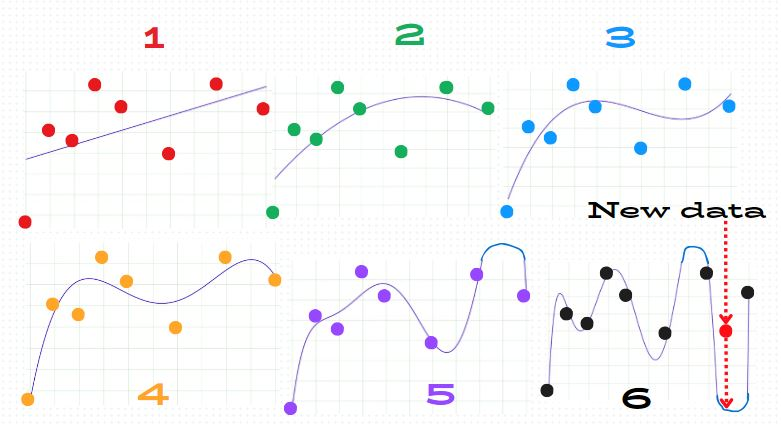
\includegraphics[width=0.75\linewidth]{img/lecture19/graphs2.JPG}
%     \caption{Example of Overfitting}
%     \label{fig:enter-label}
% \end{figure}

% \begin{itemize}
%     \item Notice in Figure 18.1 with each application of the Reconstruction Loss equation, the line fits the data better each time in graphs 1-4. However, notice in graphs 5 and 6 that overfitting takes place.  The curve swirls up and down adding noise to our curve fitting.  In graph 6, the model has memorized the exact locations of the input data.  If I were to introduce new data to this model, it would struggle to properly classify the data and yield poor performance overall.  To solve overfitting, we introduce regularization techniques for better classification and thus performance.
% \end{itemize}

\section{Regularized Autoencoders}

While basic autoencoders are effective at learning compressed representations, they often struggle with overfitting and may learn trivial identity mappings when the model has sufficient capacity. As neural networks became larger and more expressive, these limitations motivated the development of \textbf{regularized autoencoder variants}. 

Regularized autoencoders introduce additional constraints that encourage the model to learn meaningful and robust features rather than simply memorizing the training data. In this section, we explore several important extensions, including \textbf{sparse autoencoders}, \textbf{denoising autoencoders}, and \textbf{variational autoencoders}, which improve generalization and enable autoencoders to handle more complex real-world tasks.


\subsection{Regularized Autoencoders Overview}

Basic autoencoders rely on a low-dimensional bottleneck to force the network to learn compressed representations of the data. However, modern neural networks often have enough capacity to bypass this constraint and learn a trivial identity mapping, simply copying the input to the output without extracting meaningful structure. Regularized autoencoders address this limitation by encouraging the model to learn informative representations through explicit constraints on the learning process rather than relying solely on dimensionality reduction.

The key idea is that \textbf{compression is enforced through regularization instead of a small latent space}. This allows the latent representation \(Z\) to be high-dimensional while still capturing useful and generalizable features. By constraining how the encoder and decoder learn, the model is encouraged to discover structure in the data rather than memorize the training set. In this lecture, we study three major regularization strategies: \textbf{sparse autoencoders}, \textbf{denoising autoencoders}, and \textbf{variational autoencoders}.

The objective of regularization is to prevent the encoder–decoder network from learning a direct 1:1 mapping between the input and the output. Without regularization, a high-capacity autoencoder can ``cheat'' by memorizing the training data instead of learning meaningful patterns. This is analogous to memorizing answers for an exam without understanding the underlying concepts. Regularization forces the model to extract structure and learn features that generalize to new data.

\begin{figure}[H]
    \centering
    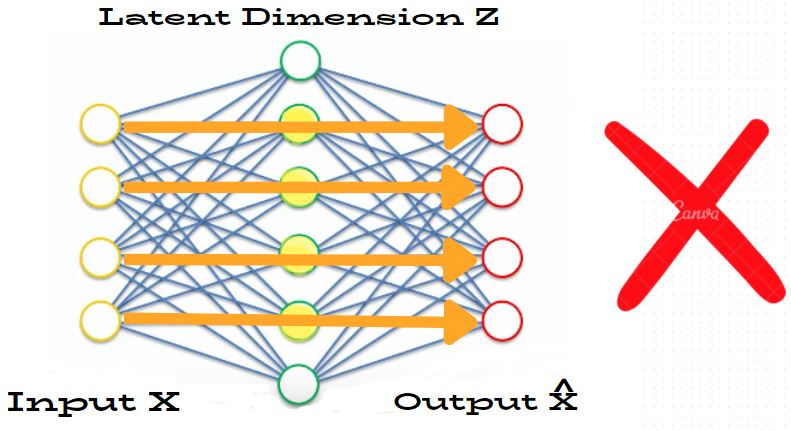
\includegraphics[width=0.5\linewidth]{img/lecture19/121mapping1.JPG}
    \caption{Figure 18.1: Regularization prevents the undesirable identity mapping and encourages the model to learn meaningful patterns.}
    \label{fig:enter-label}
\end{figure}

\paragraph{Key Takeaways}
\begin{itemize}
    \item Regularized autoencoders can use \textbf{high-dimensional latent spaces}. Representation quality is enforced by regularization rather than by a dimensional bottleneck.
    \item Regularization discourages redundant or trivial features and improves the model's ability to \textbf{generalize to unseen data}.
\end{itemize}




\subsection{Sparse Autoencoders}

Sparse autoencoders encourage the network to activate only a small subset of neurons for any given input. Instead of forcing compression through a small latent dimension, sparsity forces the model to represent each input using only a few active features. This encourages the network to discover distinctive and interpretable patterns in the data.

The key idea is that even if the latent space is large, the model is restricted in how many neurons it can use at once. As a result, the autoencoder cannot simply copy the input using all available neurons and must instead learn a compact set of meaningful features.

\paragraph{Motivation.}
Sparse representations are widely used in machine learning and neuroscience because they tend to capture the most informative structure in data. By activating only a subset of neurons during each forward pass, the model is prevented from memorizing the input and is encouraged to learn reusable features that are useful for downstream tasks such as classification and clustering.

\begin{figure}[H]
    \centering
    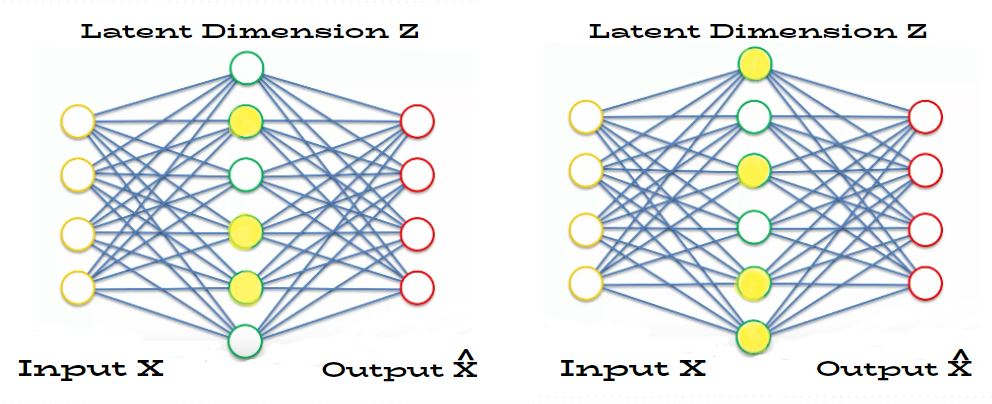
\includegraphics[width=0.75\linewidth]{img/lecture19/SparseMapping.JPG}
    \caption{Figure 18.2: Sparse autoencoders activate only a subset of neurons for any given input.}
\end{figure}

\paragraph{How sparsity is enforced.}
Sparse autoencoders introduce a regularization term into the loss function:
\[
\mathcal{L}_{\text{total}}
=
\mathcal{L}_{\text{reconstruction}}
+
\lambda \, \Omega(Z)
\]
Here, \(\mathcal{L}_{\text{reconstruction}}\) measures how accurately the decoder reconstructs the input, \(\Omega(Z)\) is a sparsity-promoting penalty applied to the latent representation \(Z\), and \(\lambda > 0\) controls the tradeoff between reconstruction quality and sparsity. A larger value of \(\lambda\) places more emphasis on sparsity, while a smaller value prioritizes reconstruction accuracy.

In other words, the model is no longer rewarded only for reconstructing well. It is also penalized if too many latent units are active. This prevents the latent representation from becoming a dense copy of the input and instead encourages the network to encode the input using only a small set of informative features.

\begin{figure}[H]
    \centering
    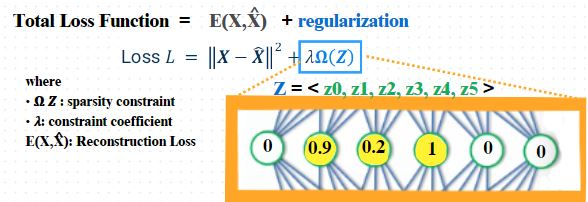
\includegraphics[width=0.75\linewidth]{img/lecture19/LossFunction4.JPG}
    \caption{Figure 18.3: Sparse autoencoders add a regularization term to the reconstruction loss.}
\end{figure}

Figure 18.3 illustrates this idea visually, but the key mathematical point is that sparsity is enforced by augmenting the reconstruction objective with an additional penalty term. Two common techniques are used to define \(\Omega(Z)\).

\paragraph{L1 Regularization on Activations.}

One simple method is to apply an \(L_1\) penalty directly to the latent activations:
\[
\Omega(Z) = \sum_{i=1}^{d} |z_i|
\]
where \(d\) is the latent dimension and \(z_i\) is the \(i\)-th latent activation for a given input. This regularizer measures the total absolute magnitude of the latent activations.

Substituting this into the sparse autoencoder objective gives:
\[
\mathcal{L}_{\text{total}}
=
\mathcal{L}_{\text{reconstruction}}
+
\lambda \sum_{i=1}^{d} |z_i|
\]

This equation shows that the model is penalized whenever many latent coordinates are active or when their magnitudes become too large. The \(L_1\) norm is well known for encouraging sparsity, so the network learns to keep most activations close to zero and rely on only a few neurons for each input. As a result, the learned representation becomes compact and selective rather than dense and redundant.

\begin{figure}[H]
    \centering
    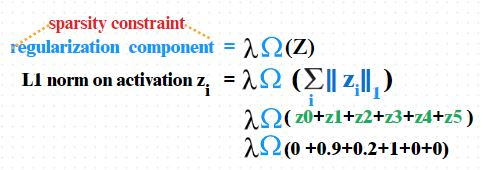
\includegraphics[width=0.55\linewidth]{img/lecture19/L1norm.JPG}
    \caption{Figure 18.4: L1 regularization encourages many latent activations to become zero.}
\end{figure}

Figure 18.4 provides the geometric intuition behind the \(L_1\) penalty. In the sparse autoencoder setting, the practical consequence is that different inputs activate different small subsets of latent units rather than spreading information across all neurons.

\paragraph{KL-Divergence Sparsity Constraint.}

Another common approach is to control the \emph{average activation} of each neuron across the training set. Let
\[
\hat{\rho}_j = \frac{1}{N}\sum_{n=1}^{N} a_j\!\left(x^{(n)}\right)
\]
denote the empirical average activation of latent neuron \(j\), where \(a_j(x^{(n)})\) is the activation of neuron \(j\) for the \(n\)-th training example and \(N\) is the number of training samples.

We then choose a small target sparsity level \(\rho\) (for example, \(\rho = 0.05\)) and encourage each neuron to satisfy
\[
\hat{\rho}_j \approx \rho.
\]
Here, \(\rho\) is the desired average activation level, while \(\hat{\rho}_j\) is the actual average activation observed during training. If \(\hat{\rho}_j\) becomes much larger than \(\rho\), then neuron \(j\) is being used too frequently and should be penalized.

This can be enforced using a KL-divergence penalty:
\[
\Omega(Z) = \sum_{j=1}^{d} D_{KL}(\rho \,\|\, \hat{\rho}_j)
\]
where
\[
D_{KL}(\rho \,\|\, \hat{\rho}_j)
=
\rho \log\frac{\rho}{\hat{\rho}_j}
+
(1-\rho)\log\frac{1-\rho}{1-\hat{\rho}_j}.
\]

The total objective therefore becomes
\[
\mathcal{L}_{\text{total}}
=
\mathcal{L}_{\text{reconstruction}}
+
\lambda \sum_{j=1}^{d} D_{KL}(\rho \,\|\, \hat{\rho}_j).
\]

This equation penalizes the model when the average activation of a latent neuron deviates too far from the desired sparsity level. Unlike the \(L_1\) penalty, which acts directly on the activations of each individual input, the KL-based penalty acts on the \emph{average behavior} of each neuron across the dataset. This encourages neurons to be active only rarely, which leads to specialization and a sparse but still distributed representation.

\begin{figure}[H]
    \centering
    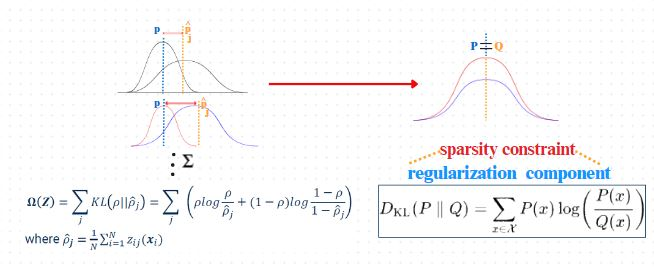
\includegraphics[width=0.9\linewidth]{img/lecture19/KL.JPG}
    \caption{Figure 18.5: KL divergence penalizes neurons that activate too frequently.}
\end{figure}

Figure 18.5 provides the intuition for the KL penalty. In practice, this encourages each latent neuron to specialize in detecting only certain structures or patterns, resulting in a sparse but still distributed representation.

\paragraph{Training.}
During training, the reconstruction loss and sparsity penalty are optimized jointly. The strength of the sparsity constraint is controlled by the hyperparameter \( \lambda \), which determines how strongly sparsity is enforced.

\begin{figure}[H]
    \centering
    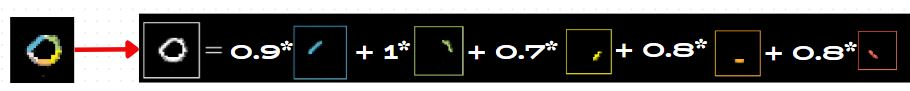
\includegraphics[width=0.75\linewidth]{img/lecture19/Sparse4.JPG}
    \caption{Figure 18.6: Sparse autoencoders represent inputs using only a few active features.}
\end{figure}

\paragraph{Key Takeaways:}
\begin{itemize}
    \item Sparse autoencoders learn representations using only a small number of active neurons.
    \item Sparsity encourages feature discovery, noise reduction, and better generalization.
    \item Sparsity can be enforced using \(L_1\) penalties or KL-divergence constraints on activations.
\end{itemize}


\subsection{Denoising Autoencoders}

Denoising autoencoders learn robust representations by training the model to reconstruct clean inputs from corrupted versions. Instead of simply copying the input, the network must learn the underlying structure of the data in order to remove noise. This encourages the encoder to capture stable and meaningful features that are useful even when the input is partially corrupted.

\paragraph{Objective}
The goal of a denoising autoencoder is to learn features that can remove noise from corrupted data. During training, noise is intentionally added to the input, and the model is asked to reconstruct the original clean version. Because the model never sees the clean input directly, it must learn the true structure of the data rather than memorizing pixel-level details.

\begin{figure}[H]
    \centering
    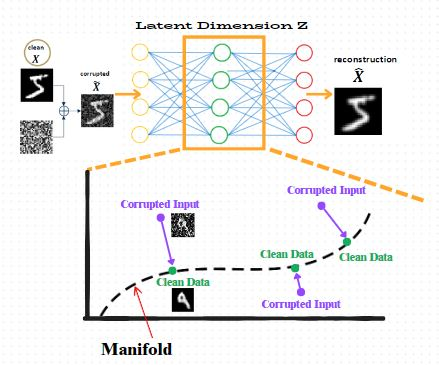
\includegraphics[width=0.65\linewidth]{img/lecture19/DeNoiseManifold.JPG}
    \caption{Figure 18.7: Denoising autoencoder: corrupted inputs are mapped back to clean outputs.}
\end{figure}

A useful way to understand denoising autoencoders is through the concept of a \emph{data manifold}. Real-world data often lies on a lower-dimensional, smooth manifold embedded in a high-dimensional space. Clean data points lie on this manifold, while noisy or corrupted inputs are pushed away from it. The denoising autoencoder learns to map corrupted inputs back to the nearest point on the learned manifold, effectively pulling noisy samples toward the region where true data lives.

\paragraph{Training Process}

During training, the input \(X\) is first corrupted to produce a noisy version \(\tilde{X}\). The encoder receives \(\tilde{X}\), not \(X\), and the decoder is trained to reconstruct the original clean input:
\[
\hat{X} = G_\phi(E_\theta(\tilde{X})).
\]
Here, \(E_\theta(\cdot)\) denotes the encoder with parameters \(\theta\), \(G_\phi(\cdot)\) denotes the decoder with parameters \(\phi\), \(\tilde{X}\) is the corrupted input, and \(\hat{X}\) is the reconstruction of the original clean sample \(X\).

A more complete way to write this is to introduce a corruption process \(q_D(\tilde{X}\mid X)\), which defines how noise is added to the clean input. The denoising autoencoder then minimizes the expected reconstruction loss:
\[
\mathcal{L}_{\text{DAE}}
=
\mathbb{E}_{\tilde{X}\sim q_D(\tilde{X}\mid X)}
\left[
\|X-\hat{X}\|_2^2
\right]
\]
with
\[
\hat{X} = G_\phi(E_\theta(\tilde{X})).
\]

In this objective, the expectation is taken over corrupted versions of the same clean input. The squared error term \(\|X-\hat{X}\|_2^2\) measures how closely the decoder recovers the original clean sample from its noisy version. Thus, the model is trained not to reproduce what it sees, but to infer the underlying clean structure from a corrupted observation.

\begin{figure}[H]
    \centering
    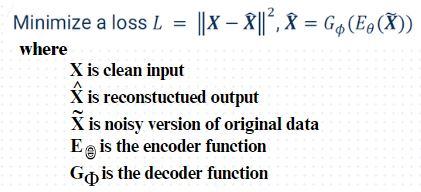
\includegraphics[width=0.5\linewidth]{img/lecture19/NoiseLoss.JPG}
    \caption{Figure 18.8: Loss function used to train a denoising autoencoder.}
\end{figure}

Figure 18.8 shows this objective visually. The important mathematical idea is that the network is not rewarded for simply reproducing its input. Instead, it must infer the clean underlying structure from a corrupted observation. This is why denoising acts as a form of regularization and leads to more robust latent features.

\paragraph{Why Denoising Works}

By learning to remove noise, the model is forced to capture stable patterns that are shared across many examples. This acts as a powerful form of regularization. The learned representation becomes robust to perturbations, small variations, and measurement errors.

\paragraph{Use Cases and Limitations}

Denoising autoencoders are widely used in image restoration, signal processing, and representation learning for noisy datasets. They are especially useful when real-world data is imperfect or corrupted.

However, denoising autoencoders do not impose strong structure on the latent space. If we randomly sample points from the latent space, there is no guarantee that they will decode into realistic data. This limitation motivates the development of \emph{variational autoencoders}, which explicitly structure the latent space for generative modeling.

\subsection{Variational Autoencoders}

Variational Autoencoders (VAEs) extend traditional autoencoders by combining representation learning with generative modeling. While standard autoencoders learn how to compress and reconstruct data, they do not impose structure on the latent space. As a result, randomly sampling from the latent space often produces unrealistic outputs. VAEs solve this problem by learning a \emph{probabilistic} latent space that is continuous, smooth, and suitable for generation.

\paragraph{Probabilistic Latent Space}

Instead of encoding each input as a single point in latent space, a VAE encodes each input as a \emph{distribution}. The encoder outputs the mean \( \mu \) and variance \( \sigma^2 \) of a Gaussian distribution that represents where the data point is likely to lie in the latent space.

\begin{figure}[H]
    \centering
    \includegraphics[width=0.5\linewidth]{img/lecture19/Structure-of-the-variational-autoencoder-VAE.png}
    \caption{Figure 18.9: Structure of a variational autoencoder. The encoder maps an input \(X\) to the parameters \(\mu\) and \(\sigma\) of the approximate posterior \(q_\theta(Z|X)\). A latent code \(Z\) is sampled from this distribution and passed through the decoder \(p_\phi(X|Z)\) to reconstruct the input.}
\end{figure}

Sampling from these distributions produces latent points that are close to one another in a continuous manner. This continuity allows smooth interpolation between data points and enables the model to generate realistic new samples.

\paragraph{Generative Modeling View}

VAEs model the data using a latent-variable generative process. First, a latent code is sampled from a prior distribution:
\[
Z \sim p(Z),
\]
and then an observation is generated from the decoder likelihood:
\[
X \sim p_\phi(X|Z).
\]

Equivalently, the joint distribution can be written as
\[
p_\phi(X,Z)=p(Z)\,p_\phi(X|Z).
\]
Here, \(p(Z)\) is the prior distribution over latent variables, \(p_\phi(X|Z)\) is the decoder likelihood that describes how data is generated from a latent code, and \(p_\phi(X,Z)\) is the joint probability of simultaneously observing both \(X\) and \(Z\).

The prior \(p(Z)\) is usually chosen to be a standard Gaussian:
\[
p(Z)=\mathcal{N}(0,I),
\]
because it is simple to sample from and encourages a smooth latent space.

To evaluate how likely an observed data point \(X\) is under the model, we marginalize over all possible latent variables:
\[
p_\phi(X)=\int p_\phi(X,Z)\,dZ
=
\int p(Z)\,p_\phi(X|Z)\,dZ.
\]

This equation says that the probability of observing \(X\) is obtained by summing, or more precisely integrating, over all latent codes \(Z\) that could have generated it. This marginal likelihood is the quantity we would ideally like to maximize during training, because doing so encourages the model to assign high probability to the observed data and thus learn to generate realistic samples.

\paragraph{Why Direct Likelihood is Intractable}

The main difficulty is that the marginal likelihood
\[
p_\phi(X)=\int p(Z)\,p_\phi(X|Z)\,dZ
\]
requires us to integrate over \emph{all possible} latent values \(Z\) that could explain the observed data point \(X\). In other words, even for a single input \(X\), there is not just one possible latent explanation. There may be infinitely many candidate latent codes \(Z\) that could plausibly generate the same observation.

This is similar in spirit to the intuition behind Figure 18.2, where multiple possible feature activations may contribute to a representation. Here, however, the issue is probabilistic: instead of choosing one latent code, we must consider \emph{every possible} latent code and weigh how likely each one is under the prior \(p(Z)\) and the decoder likelihood \(p_\phi(X|Z)\).

In low-dimensional settings, such an integral may sometimes be manageable, but in high-dimensional latent spaces there are infinitely many candidate latent configurations, and the integral typically has no closed-form solution. Therefore, directly computing
\[
p_\phi(X)=\int p(Z)\,p_\phi(X|Z)\,dZ
\]
is generally intractable.

This also makes the true posterior distribution difficult to compute:
\[
p_\phi(Z|X)=\frac{p_\phi(X|Z)p(Z)}{p_\phi(X)}.
\]
The denominator \(p_\phi(X)\) is exactly the same intractable marginal likelihood above. Therefore, if we cannot compute \(p_\phi(X)\), then we also cannot compute the exact posterior efficiently.

VAEs address this problem by introducing an approximate posterior distribution \(q_\theta(Z|X)\) and replacing exact inference with a tractable optimization procedure called \emph{variational inference}.

\paragraph{Variational Inference and the ELBO}

Since the true posterior \(p_\phi(Z|X)\) is intractable, VAEs introduce an approximate posterior \(q_\theta(Z|X)\), parameterized by the encoder. This approximation is chosen from a simpler family of distributions, and the goal is to make it as close as possible to the true posterior.

This idea is called \textbf{variational inference}. Instead of trying to compute the exact posterior \(p_\phi(Z|X)\) directly, variational inference replaces it with a simpler distribution \(q_\theta(Z|X)\) and then optimizes the parameters of that distribution so that it approximates the true posterior as closely as possible.

Rather than maximizing \(\log p_\phi(X)\) directly, we maximize a tractable lower bound called the \emph{Evidence Lower Bound (ELBO)}:
\[
\mathcal{L}_{\text{ELBO}}(X)
=
\mathbb{E}_{q_\theta(Z|X)}[\log p_\phi(X|Z)]
-
D_{KL}\!\left(q_\theta(Z|X)\|p(Z)\right).
\]

Here, \(q_\theta(Z|X)\) is the encoder distribution, \(p_\phi(X|Z)\) is the decoder likelihood, and \(p(Z)\) is the latent prior. The expectation \(\mathbb{E}_{q_\theta(Z|X)}[\cdot]\) means that the reconstruction quality is averaged over latent samples drawn from the encoder distribution.

\begin{figure}[H]
    \centering
    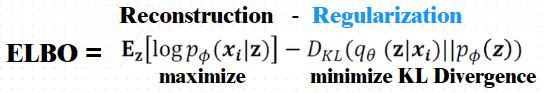
\includegraphics[width=0.70\linewidth]{img/lecture19/ELBO2.JPG}
    \caption{Figure 18.10: Evidence Lower Bound (ELBO) objective.}
\end{figure}

Unlike a standard autoencoder that maps each input to a single latent vector, a VAE maps each input to a distribution in latent space, meaning that one observed sample can have many plausible latent explanations.

This objective has two components:
\[
\mathcal{L}_{\text{ELBO}}(X)
=
\underbrace{\mathbb{E}_{q_\theta(Z|X)}[\log p_\phi(X|Z)]}_{\text{reconstruction / likelihood term}}
-
\underbrace{D_{KL}\!\left(q_\theta(Z|X)\|p(Z)\right)}_{\text{regularization term}}.
\]

The first term is the \textbf{reconstruction term}, which is also the decoder \textbf{likelihood function}. This plays a role similar to likelihood functions studied earlier in probabilistic models such as Naive Bayes, where we evaluate how probable the observed data is under a model. Here, the decoder learns to assign high likelihood to the observed data \(X\) given the latent variable \(Z\), which encourages accurate reconstruction.

The second term is the \textbf{regularization term}, which is a KL divergence. This connects to earlier discussions of KL divergence as a measure of how different two distributions are, such as in clustering and distribution comparison. Here, the KL term forces the encoder distribution \(q_\theta(Z|X)\) to remain close to the prior \(p(Z)\). This prevents the latent space from becoming irregular or fragmented and instead encourages a smooth and well-structured latent representation.

Thus, the ELBO can be interpreted as balancing two goals: maximizing likelihood (good reconstruction) while minimizing distribution mismatch (good latent structure). In this way, variational inference turns an intractable probabilistic inference problem into an optimization problem: instead of computing the exact posterior, we optimize the ELBO so that \(q_\theta(Z|X)\) becomes a useful approximation to \(p_\phi(Z|X)\).

\paragraph{Reparameterization Trick}

Training VAEs requires gradients to pass through the sampling step. However, direct sampling
\[
Z \sim \mathcal{N}(\mu,\sigma^2)
\]
introduces stochasticity in a way that prevents standard backpropagation through \(\mu\) and \(\sigma\). Here, \(\mu\) and \(\sigma^2\) are the mean and variance predicted by the encoder for a given input.

To resolve this, VAEs use the \emph{reparameterization trick}, rewriting the latent sample as
\[
Z = \mu + \sigma \odot \epsilon,
\qquad
\epsilon \sim \mathcal{N}(0,I),
\]
where \(\epsilon\) contains the randomness and \(\mu,\sigma\) are deterministic outputs of the encoder.

In this form, the randomness is isolated in \(\epsilon\), while \(Z\) becomes a differentiable function of \(\mu\) and \(\sigma\). This allows gradients to flow through the encoder parameters during training, making end-to-end optimization with backpropagation possible.

\begin{figure}[H]
    \centering
    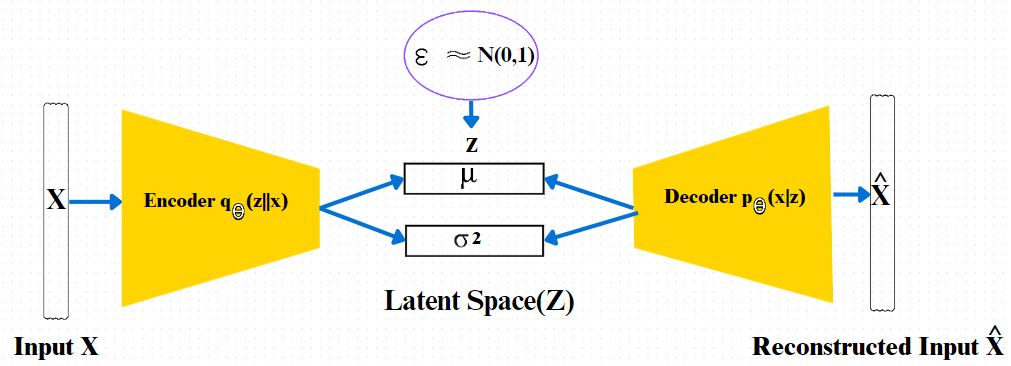
\includegraphics[width=0.85\linewidth]{img/lecture19/Trick2.JPG}
    \caption{Figure 18.11: Reparameterization trick for gradient-based training.}
\end{figure}

\paragraph{Reconstruction and Generation Modes}

Because the latent space is probabilistic and structured, VAEs support two modes of operation. During reconstruction, an input is encoded into a distribution and decoded back to recreate the original data. During generation, we bypass the encoder and directly sample from the latent prior to create new data.

\begin{figure}[H]
    \centering
    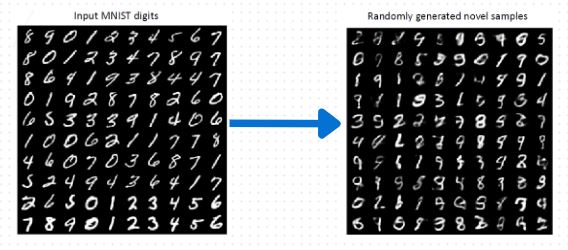
\includegraphics[width=0.65\linewidth]{img/lecture19/NovelSamples.JPG}
    \caption{Figure 18.12: Generation mode: sampling from latent space.}
\end{figure}

\paragraph{Smooth Interpolation in Latent Space}

The Gaussian prior encourages nearby latent points to decode into similar outputs. Moving smoothly through latent space therefore produces gradual and realistic changes in generated data.

\begin{figure}[H]
    \centering
    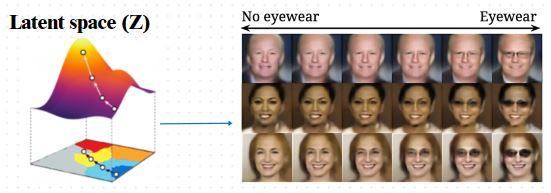
\includegraphics[width=0.75\linewidth]{img/lecture19/VAEMorphing1.JPG}
    \caption{Figure 18.13: Smooth transitions in VAE latent space.}
\end{figure}

\paragraph{Key Advantages}

VAEs provide a principled framework for learning meaningful latent representations while enabling realistic data generation. They support interpolation, anomaly detection, and unsupervised representation learning, making them a powerful extension of traditional autoencoders.

% \section{Summary}
% \hspace{1.3em}
% Autoencoders are unsupervised neural networks designed to learn efficient data representations by encoding input data into a compressed latent space and then reconstructing it as closely as possible at the output. While basic autoencoders focus solely on minimizing reconstruction error, regularized variations introduce additional constraints that enhance their utility and versatility. L1 regularization encourages sparsity in the latent space, making the model focus on key features and filter out noise. KL divergence regularization, often used in sparse and variational autoencoders, enforces a specific distribution (typically Gaussian) on the latent space, creating a structured and continuous space that is useful for generation and interpretability. Denoising autoencoders add robustness by training the model to reconstruct clean data from noisy inputs, improving generalization and noise tolerance. Variational autoencoders (VAEs) take this a step further by using probabilistic sampling in the latent space, allowing for smooth interpolation between data points and the generation of novel, realistic outputs. Together, these variations extend the foundational autoencoder’s capabilities, making it applicable in feature extraction, dimensionality reduction, data generation, and anomaly detection. Each regularization approach refines the autoencoder's performance to fit specific tasks, whether through sparsity, structured continuity, robustness, or generative power.


\section{Summary}

Regularized autoencoders extend basic autoencoders by introducing constraints that prevent trivial identity mapping and encourage meaningful feature learning.

\paragraph{Key Takeaways}
\begin{itemize}
    \item Basic autoencoders rely on dimensional bottlenecks, while regularized autoencoders enforce structure through additional loss terms.
    \item \textbf{Sparse autoencoders} encourage feature discovery by activating only a small subset of neurons.
    \item \textbf{Denoising autoencoders} learn robust representations by reconstructing clean data from corrupted inputs.
    \item \textbf{Variational autoencoders (VAEs)} introduce a probabilistic latent space, enabling generation of new data and smooth interpolation.
    \item Regularized autoencoders are widely used for representation learning, dimensionality reduction, anomaly detection, and generative modeling.
\end{itemize}


\section{Q \& A Section}

\begin{enumerate}

\item \textbf{Question:} 
Why can a standard autoencoder fail when the latent dimension is large?

\textbf{Solution:}  
If the latent space is large, the network has enough capacity to simply copy the input to the output. Instead of learning meaningful structure, it learns a near identity mapping. This limits its usefulness for representation learning because the model memorizes the data instead of extracting meaningful features. Regularization techniques such as sparsity, noise injection, or probabilistic constraints help prevent this behavior.

\item \textbf{Question:} 
How does a sparse autoencoder address this issue?

\textbf{Solution:}  
Sparse autoencoders add a penalty that forces most latent neurons to remain inactive. Because only a few neurons can activate at once, the model must learn efficient and informative features instead of copying the entire input. This encourages feature discovery and improves generalization.

\item \textbf{Question:} 
What is the main idea behind denoising autoencoders?

\textbf{Solution:}  
Denoising autoencoders are trained on corrupted inputs but must reconstruct the original clean data. This forces the network to learn stable patterns that reflect the underlying structure of the data rather than memorizing pixel-level details. As a result, the learned representation becomes more robust to noise and perturbations.

\item \textbf{Question:} 
Why are basic autoencoders not suitable for generating new data?

\textbf{Solution:}  
The latent space in a basic autoencoder is not structured or constrained to follow any particular distribution. Randomly sampling from this space may produce unrealistic outputs because there is no guarantee that sampled points correspond to valid data. Variational autoencoders solve this by enforcing a structured latent distribution.

\item \textbf{Question:} 
What distinguishes a Variational Autoencoder (VAE) from other autoencoder variants?

\textbf{Solution:}  
A VAE models the latent space probabilistically and enforces a structured distribution (typically Gaussian). Instead of mapping each input to a single latent vector, the encoder produces a distribution defined by a mean and variance. This makes the latent space continuous and smooth, allowing meaningful sampling and generation of new data.

\item \textbf{Question:}
Why is direct maximum likelihood training difficult in VAEs?

\textbf{Solution:}

VAEs attempt to maximize the marginal likelihood:
\[
p_\phi(x) = \int p_\phi(x|z)p(z)\,dz
\]
This requires integrating over all possible latent variables \(z\). Since the latent space is typically high dimensional, this integral is computationally intractable. The posterior
\[
p_\phi(z|x)=\frac{p_\phi(x|z)p(z)}{p_\phi(x)}
\]
is also difficult to compute because it depends on the same intractable quantity \(p_\phi(x)\).

\item \textbf{Question:}
What is variational inference in VAEs?

\textbf{Solution:}

Variational inference replaces the true posterior \(p_\phi(z|x)\) with a simpler approximation \(q_\theta(z|x)\). Instead of solving the exact inference problem, we optimize \(q_\theta(z|x)\) so that it becomes close to the true posterior. In practice, this turns posterior inference into an optimization problem that can be solved efficiently.

\item \textbf{Question:}
Derive the Evidence Lower Bound (ELBO) in a compact form.

\textbf{Solution:}

Start with the log likelihood:
\[
\log p_\phi(x)
=
\log \int q_\theta(z|x)\frac{p_\phi(x,z)}{q_\theta(z|x)}\,dz
\]

Rewrite it as an expectation:
\[
\log p_\phi(x)
=
\log
\mathbb{E}_{q_\theta(z|x)}
\left[
\frac{p_\phi(x,z)}{q_\theta(z|x)}
\right]
\]

Apply Jensen's inequality:
\[
\log p_\phi(x)
\ge
\mathbb{E}_{q_\theta(z|x)}
\left[
\log \frac{p_\phi(x,z)}{q_\theta(z|x)}
\right]
\]

Expand \(p_\phi(x,z)=p_\phi(x|z)p(z)\):
\[
\log p_\phi(x)
\ge
\mathbb{E}_{q_\theta(z|x)}[\log p_\phi(x|z)]
+
\mathbb{E}_{q_\theta(z|x)}[\log p(z)-\log q_\theta(z|x)]
\]

Thus,
\[
\mathcal{L}_{ELBO}
=
\mathbb{E}_{q_\theta(z|x)}[\log p_\phi(x|z)]
-
D_{KL}(q_\theta(z|x)\|p(z))
\]

This is called the Evidence Lower Bound because it is a lower bound on \(\log p_\phi(x)\).

\item \textbf{Question:}
What do the two ELBO terms represent intuitively?

\textbf{Solution:}

The ELBO contains two parts:
\[
\mathbb{E}_{q_\theta(z|x)}[\log p_\phi(x|z)]
\]
is the reconstruction or likelihood term. It encourages the decoder to assign high probability to the observed data, given the latent representation. This is the part responsible for accurate reconstruction.

\[
D_{KL}(q_\theta(z|x)\|p(z))
\]
is the regularization term. It keeps the learned latent distribution close to the prior \(p(z)\), which helps create a smooth and structured latent space. Thus, in the ELBO, reconstruction comes from the likelihood function, while regularization comes from KL divergence.

\item \textbf{Question:}
Why is the reparameterization trick necessary?

\textbf{Solution:}

If we sample directly as
\[
z \sim \mathcal{N}(\mu,\sigma^2),
\]
then the sampling operation blocks gradient flow. To make backpropagation possible, we rewrite the sample as
\[
z = \mu + \sigma \epsilon,
\qquad \epsilon \sim \mathcal{N}(0,1)
\]
Now the randomness is isolated in \(\epsilon\), while \(\mu\) and \(\sigma\) remain inside a differentiable expression. This allows gradients to flow through the encoder parameters during training.

\item \textbf{Question:}
Why does KL regularization help produce a smooth latent space?

\textbf{Solution:}

The KL term forces the approximate posterior \(q_\theta(z|x)\) to remain close to a simple prior such as \(\mathcal{N}(0,I)\). This prevents the latent codes from becoming arbitrarily scattered or forming disconnected regions. As a result, nearby points in latent space tend to decode into similar outputs, enabling smooth interpolation and meaningful sampling.

\end{enumerate}


\section{References}

\begin{itemize}

\item See Figure 18.1 for the image adapted from Yadav, S. (n.d.). Overfitting and regularization in machine learning. Towards Data Science. \url{https://towardsdatascience.com/over-fitting-and-regularization-64d16100f45c}

\item See Figures 18.2 and 18.3 for the image adapted from Data School. (n.d.). Autoencoders in deep learning [Video]. YouTube. \url{https://www.youtube.com/watch?v=CiexUMrNtBQ}

\item See Figure 18.4 for the image adapted from StatQuest with Josh Starmer. (n.d.). Regularization and overfitting [Video]. YouTube. \url{https://www.youtube.com/watch?v=xwrzh4e8DLs}

\item See Figure 18.5 for the image adapted from Chorri, M. (n.d.). Difference between KL divergence and PSI. Medium. \url{https://medium.com/@mumbaiyachori/difference-between-kl-divergence-and-psi-e7d9aa0ade12}

\item See Figure 18.6 for the image adapted from Saturn Cloud. (n.d.). Sparse autoencoders. \url{https://saturncloud.io/glossary/sparse-autoencoders/}

\item See Figures 18.7 and 18.8 for the image adapted from 3Blue1Brown. (n.d.). Neural networks: How they work [Video]. YouTube. \url{https://www.youtube.com/watch?v=aircAruvnKk}

\item See Figure 18.9 for the image adapted from Abdelli, K., Griesser, H., Neumeyr, C., et al. (2022, November). \textit{Degradation Prediction of Semiconductor Lasers using Conditional Variational Autoencoder} (preprint available via ResearchGate). \url{https://www.researchgate.net/figure/Structure-of-the-variational-autoencoder-VAE_fig1_365190062}

\item See Figures 18.10 and 18.11 for the image adapted from Krasser, F. (2018). Latent space optimization. \url{https://krasserm.github.io/2018/04/07/latent-space-optimization/}

\item See Figure 18.12 for the image adapted from Bose, S. (n.d.). Comparison of autoencoders vs. variational autoencoders. Medium. \url{https://medium.com/@jwbtmf/comparison-of-autoencoders-vs-variational-autoencoders-7993442bb377}

\item See Figure 18.13 for the image adapted from Van Rensburg, E. (n.d.). Generating the intuition behind variational autoencoders (VAEs). Medium. \url{https://medium.com/@elzettevanrensburg/generating-the-intuition-behind-variational-auto-encoders-vaes-c7d2f8631a87}

\item Schafer, A. (n.d.). L1 norm, regularization, and sparsity explained for dummies. ML Review. \url{https://blog.mlreview.com/l1-norm-regularization-and-sparsity-explained-for-dummies-5b0e4be3938a}

\item Rathi, M. (n.d.). Neural network terminology explained. Mukul Rathi. \url{https://mukulrathi.com/demystifying-deep-learning/neural-network-terminology-explained/}

\item Two Minute Papers. (n.d.). The future of deep learning research [Video]. YouTube. \url{https://www.youtube.com/watch?v=b8AzCgY1gZI}

\item deeplearning.ai. (n.d.). Deep learning explained [Video]. YouTube. \url{https://www.youtube.com/watch?v=2859tNY-G5E}

\item Mandal, S. (n.d.). Difference between overfitting and underfitting in machine learning. Medium. \url{https://medium.com/@soumallya160/difference-of-overfitting-underfitting-7f0bd08fb8a6}

\item Kingma, D. P., and Welling, M. (2014). Auto-Encoding Variational Bayes. \textit{International Conference on Learning Representations (ICLR)}. \url{https://arxiv.org/abs/1312.6114}

\item Murphy, K. P. (2022). \textit{Probabilistic Machine Learning: An Introduction}. MIT Press.

\item Bishop, C. M. (2006). \textit{Pattern Recognition and Machine Learning}. Springer.

\end{itemize}


% \section{References}
% % \subsection{List of Resources Used}

% \begin{itemize}

% \item See Figure 18.14 for the image sourced from Khan Academy. (n.d.). What is an autoencoder? [Video]. YouTube. \url{https://www.youtube.com/watch?v=iwEzwTTalbg}

% \item See Figure 18.8 for the image sourced from 3Blue1Brown. (n.d.). Neural networks: How they work [Video]. YouTube. \url{https://www.youtube.com/watch?v=aircAruvnKk}

% \item deeplearning.ai. (n.d.). Deep learning explained [Video]. YouTube. \url{https://www.youtube.com/watch?v=2859tNY-G5E}

% \item See Figure 18.2, 18.3, 18.9, and 18.11 for the image sourced from Data School. (n.d.). Autoencoders in deep learning [Video]. YouTube. \url{https://www.youtube.com/watch?v=CiexUMrNtBQ}

% \item Two Minute Papers. (n.d.). The future of deep learning research [Video]. YouTube. \url{https://www.youtube.com/watch?v=b8AzCgY1gZI}

% \item See Figure 18.4 for the image sourced from StatQuest with Josh Starmer. (n.d.). Regularization and overfitting [Video]. YouTube. \url{https://www.youtube.com/watch?v=xwrzh4e8DLs}


% \item Saturn Cloud. (n.d.). Sparse autoencoders. \url{https://saturncloud.io/glossary/sparse-autoencoders/}

% \sloppy
% \item Schafer, A. (n.d.). L1 norm, regularization, and sparsity explained for dummies. ML Review. \url{https://blog.mlreview.com/l1-norm-regularization-and-sparsity-explained-for-dummies-5b0e4be3938a}

% \sloppy
% \item Rathi, M. (n.d.). Neural network terminology explained. Mukul Rathi. \url{https://mukulrathi.com/demystifying-deep-learning/neural-network-terminology-explained/}


% \item See Figure 18.1 for the image sourced from Yadav, S. (n.d.). Overfitting and regularization in machine learning. Towards Data Science. \url{https://towardsdatascience.com/over-fitting-and-regularization-64d16100f45c}


% \item Chorri, M. (n.d.). Difference between KL divergence and PSI. Medium. \url{https://medium.com/@mumbaiyachori/difference-between-kl-divergence-and-psi-e7d9aa0ade12}

% \item Çaglar, M. (2020, September 10). Kullback-Leibler divergence explained [Post]. X. \url{https://x.com/caglarml/status/1304051370367094787}


% \item See Figure 18.7 for the image sourced from Ryan, G. (2022, October 1). Kullback-Leibler divergence: The origin of a key concept in information theory [Post]. LinkedIn. \url{https://www.linkedin.com/posts/gabriel-ryan-frm-ba304915_kullback-liebler-divergence-the-origin-of-activity-6978629222726578178-wAUy}

% \item See Figure 18.17 for the image sourced from Van Rensburg, E. (n.d.). Generating the intuition behind variational autoencoders (VAEs). Medium. \url{https://medium.com/@elzettevanrensburg/generating-the-intuition-behind-variational-auto-encoders-vaes-c7d2f8631a87}


% \item See Figure 18.13 for the image sourced from Ram, A. (n.d.). Bayes theorem with conditional probability. Medium. \url{https://medium.com/@ram420/bayes-theorem-with-conditional-probability-793bf9caba92}

% \item See Figure 18.6, 18.11 and 18.17 for the image sourced from Krasser, F. (2018, April 7). Latent space optimization. \url{https://krasserm.github.io/2018/04/07/latent-space-optimization/}

% \item Bose, S. (n.d.). Comparison of autoencoders vs. variational autoencoders. Medium. \url{https://medium.com/@jwbtmf/comparison-of-autoencoders-vs-variational-autoencoders-7993442bb377}

% \item Mandal, S. (n.d.). Difference between overfitting and underfitting in machine learning. Medium. \url{https://medium.com/@soumallya160/difference-of-overfitting-underfitting-7f0bd08fb8a6}

% \item alregib2024neural] @miscalregib2024neural, author = Ghassan AlRegib and Mohit Prabhushankar, title =
% Lecture 18: Autoencoders, year = 2024, howpublished = ECE 4803/8803: Fundamentals of Machine
% Learning (FunML), Georgia Institute of Technology, Lecture Notes, note = Available from FunML course
% materials

% \item See Figure 18.9, 18.15 and 18.16 for the image sourced from alregib2024neural] @miscalregib2024neural, author = Ghassan AlRegib and Mohit Prabhushankar, title =
%  Lecture 19: Autoencoder Extensions, year = 2024, howpublished = ECE 4803/8803: Fundamentals of Machine
% Learning (FunML), Georgia Institute of Technology, Lecture Notes, note = Available from FunML course
% materials

% \end{itemize}

% \section{Common Notations}

% \begin{multicols}{2}
% \begin{itemize}
% \item $\mathbf{b}$: Bias vector
% \item $C_k$: K-th cluster
% \item $d(\mathbf{x_j, x_k})$: Dissimilarity between $\mathbf{x_j, x_k}$
% \item $E_\theta$: Encoding function
% \item $f(\cdot)$: Trained neural network
% \item $\mathbf{G}(t)$: Second moment at time t
% \item $G_\Phi$: Decoding function
% \item $\mathbf{H(\theta)}$: Hessian matrix
% \item $h_i, h_j$: Representation space vectors
% \item $k^{(i)}$: Number of neurons in the $i^{th}$ layer
% \item $M$: Number of features in a feature vector
% \item $m$: Degree of polynomial
% \item $m_j$: J-th centroid
% \item $N$: Number of data samples
% \item $P$: Predicted class
% \item $P^{(k)}$: The number of neurons in layer k
% \item $Q$: Contrast class
% \item $Q_k$: Computed clustering for k-th cluster
% \item $R_k$: Ground truth clustering for k-th cluster
% \item $s(\mathbf{x_j, x_k})$: Similarity between $\mathbf{x_j, x_k}$
% \item $v(t)$: First moment at time t
% \item $\mathbf{W}$: Weight matrix
% \item $w_{ij}$: Degree of membership of $\mathbf{x_i}$ in $C_j$
% \item $\mathbf{X}$: Matrix of feature vectors (dataset)
% \item $\mathbf{\hat{X}}$: Reconstruction of data
% \item $\widetilde{\mathbf{X}}$: Corrupted input
% \item $\mathbf{x_i}$: Feature vector (a data sample)
% \item $\mathbf{x_{:,i}}$: Feature vector of all data samples
% \item $x_i$: A single feature
% \item $\mathbf{Y}$: Output matrix
% \item $y_i$: Target class
% \item $y^{c}$: Predicted logit for class P
% \item $y^{i}$: Logit for any class i
% \item $\mathbf{Z}$: Latent representation
% \item \textls[-20]{$z_i$: Latent variables representing the embedding of $\mathbf{x_i}$}
% \item $\alpha$: Learning rate
% \item $\gamma$: Bias factor
% \item $\gamma_i^j$: Posterior of $\mathbf{x_i}$ coming from cluster j
% \item $\epsilon$: Error margin
% \item $\tilde{\lambda_j}$: Average activation of neuron $z_{ij}$
% \item $\boldsymbol{\theta}$: Coefficient vector
% \item $\theta_i$: A single model coefficient (parameter)
% \item $\hat{\rho_j}$: Average activation of neuron $z_{ij}$
% \item $\mathbf{\Omega(Z)}$: Sparsity constraint

% \end{itemize}
% \end{multicols}

\end{document}
